\definecolor{rsblue}{HTML}{2563EB}
\definecolor{rsgreen}{HTML}{15803D}
\definecolor{rsred}{HTML}{DC2626}
\definecolor{rsgray}{HTML}{6B7280}
\definecolor{rsgridgray}{HTML}{E5E7EB}
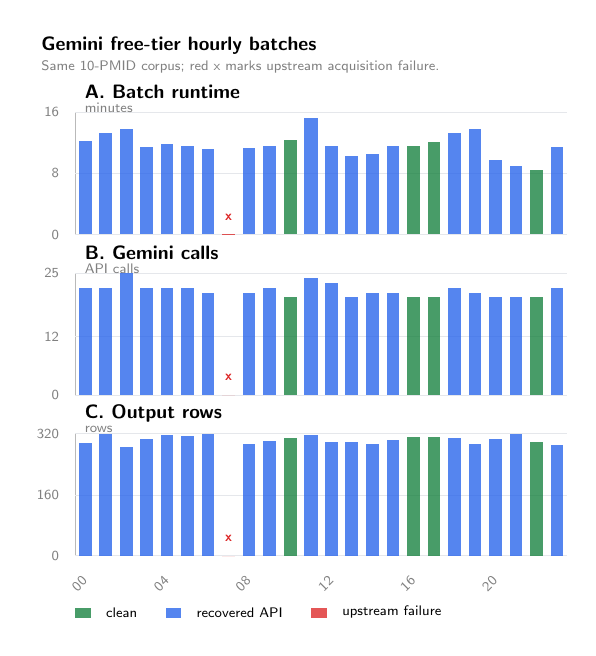
\begin{tikzpicture}[x=1cm,y=1cm,
    rsaxis/.style={draw=gray!55, line width=0.35pt},
    rsgrid/.style={draw=rsgridgray, line width=0.25pt},
    every node/.style={font=\sffamily}]
\node[anchor=west, font=\sffamily\scriptsize\bfseries] at (0,6.82) {Gemini free-tier hourly batches};
\node[anchor=west, font=\sffamily\tiny, text=gray] at (0,6.55) {Same 10-PMID corpus; red x marks upstream acquisition failure.};
\node[anchor=west, font=\sffamily\scriptsize\bfseries] at (0.55,6.23) {A. Batch runtime};
\draw[rsaxis] (0.55,4.42) -- (0.55,5.97);
\draw[rsaxis] (0.55,4.42) -- (6.80,4.42);
\draw[rsgrid] (0.55,4.42) -- (6.80,4.42);
\node[anchor=east, text=gray, font=\sffamily\tiny] at (0.47,4.42) {0};
\draw[rsgrid] (0.55,5.20) -- (6.80,5.20);
\node[anchor=east, text=gray, font=\sffamily\tiny] at (0.47,5.20) {8};
\draw[rsgrid] (0.55,5.97) -- (6.80,5.97);
\node[anchor=east, text=gray, font=\sffamily\tiny] at (0.47,5.97) {16};
\node[anchor=west, text=gray, font=\sffamily\tiny] at (0.55,6.03) {minutes};
\draw[draw=none, fill=rsblue, opacity=0.78] (0.60,4.42) rectangle (0.76,5.61);
\draw[draw=none, fill=rsblue, opacity=0.78] (0.86,4.42) rectangle (1.02,5.71);
\draw[draw=none, fill=rsblue, opacity=0.78] (1.12,4.42) rectangle (1.28,5.76);
\draw[draw=none, fill=rsblue, opacity=0.78] (1.38,4.42) rectangle (1.54,5.53);
\draw[draw=none, fill=rsblue, opacity=0.78] (1.64,4.42) rectangle (1.80,5.57);
\draw[draw=none, fill=rsblue, opacity=0.78] (1.90,4.42) rectangle (2.06,5.54);
\draw[draw=none, fill=rsblue, opacity=0.78] (2.16,4.42) rectangle (2.32,5.50);
\draw[draw=none, fill=rsred, opacity=0.78] (2.42,4.42) rectangle (2.58,4.43);
\node[text=rsred, font=\sffamily\tiny\bfseries] at (2.50,4.64) {x};
\draw[draw=none, fill=rsblue, opacity=0.78] (2.68,4.42) rectangle (2.84,5.52);
\draw[draw=none, fill=rsblue, opacity=0.78] (2.94,4.42) rectangle (3.10,5.55);
\draw[draw=none, fill=rsgreen, opacity=0.78] (3.20,4.42) rectangle (3.37,5.62);
\draw[draw=none, fill=rsblue, opacity=0.78] (3.46,4.42) rectangle (3.63,5.90);
\draw[draw=none, fill=rsblue, opacity=0.78] (3.72,4.42) rectangle (3.89,5.55);
\draw[draw=none, fill=rsblue, opacity=0.78] (3.98,4.42) rectangle (4.15,5.42);
\draw[draw=none, fill=rsblue, opacity=0.78] (4.25,4.42) rectangle (4.41,5.44);
\draw[draw=none, fill=rsblue, opacity=0.78] (4.51,4.42) rectangle (4.67,5.54);
\draw[draw=none, fill=rsgreen, opacity=0.78] (4.77,4.42) rectangle (4.93,5.54);
\draw[draw=none, fill=rsgreen, opacity=0.78] (5.03,4.42) rectangle (5.19,5.59);
\draw[draw=none, fill=rsblue, opacity=0.78] (5.29,4.42) rectangle (5.45,5.71);
\draw[draw=none, fill=rsblue, opacity=0.78] (5.55,4.42) rectangle (5.71,5.76);
\draw[draw=none, fill=rsblue, opacity=0.78] (5.81,4.42) rectangle (5.97,5.36);
\draw[draw=none, fill=rsblue, opacity=0.78] (6.07,4.42) rectangle (6.23,5.29);
\draw[draw=none, fill=rsgreen, opacity=0.78] (6.33,4.42) rectangle (6.49,5.24);
\draw[draw=none, fill=rsblue, opacity=0.78] (6.59,4.42) rectangle (6.75,5.53);
\node[anchor=west, font=\sffamily\scriptsize\bfseries] at (0.55,4.19) {B. Gemini calls};
\draw[rsaxis] (0.55,2.38) -- (0.55,3.93);
\draw[rsaxis] (0.55,2.38) -- (6.80,2.38);
\draw[rsgrid] (0.55,2.38) -- (6.80,2.38);
\node[anchor=east, text=gray, font=\sffamily\tiny] at (0.47,2.38) {0};
\draw[rsgrid] (0.55,3.12) -- (6.80,3.12);
\node[anchor=east, text=gray, font=\sffamily\tiny] at (0.47,3.12) {12};
\draw[rsgrid] (0.55,3.93) -- (6.80,3.93);
\node[anchor=east, text=gray, font=\sffamily\tiny] at (0.47,3.93) {25};
\node[anchor=west, text=gray, font=\sffamily\tiny] at (0.55,3.99) {API calls};
\draw[draw=none, fill=rsblue, opacity=0.78] (0.60,2.38) rectangle (0.76,3.74);
\draw[draw=none, fill=rsblue, opacity=0.78] (0.86,2.38) rectangle (1.02,3.74);
\draw[draw=none, fill=rsblue, opacity=0.78] (1.12,2.38) rectangle (1.28,3.93);
\draw[draw=none, fill=rsblue, opacity=0.78] (1.38,2.38) rectangle (1.54,3.74);
\draw[draw=none, fill=rsblue, opacity=0.78] (1.64,2.38) rectangle (1.80,3.74);
\draw[draw=none, fill=rsblue, opacity=0.78] (1.90,2.38) rectangle (2.06,3.74);
\draw[draw=none, fill=rsblue, opacity=0.78] (2.16,2.38) rectangle (2.32,3.68);
\draw[draw=none, fill=rsred, opacity=0.78] (2.42,2.38) rectangle (2.58,2.38);
\node[text=rsred, font=\sffamily\tiny\bfseries] at (2.50,2.60) {x};
\draw[draw=none, fill=rsblue, opacity=0.78] (2.68,2.38) rectangle (2.84,3.68);
\draw[draw=none, fill=rsblue, opacity=0.78] (2.94,2.38) rectangle (3.10,3.74);
\draw[draw=none, fill=rsgreen, opacity=0.78] (3.20,2.38) rectangle (3.37,3.62);
\draw[draw=none, fill=rsblue, opacity=0.78] (3.46,2.38) rectangle (3.63,3.87);
\draw[draw=none, fill=rsblue, opacity=0.78] (3.72,2.38) rectangle (3.89,3.81);
\draw[draw=none, fill=rsblue, opacity=0.78] (3.98,2.38) rectangle (4.15,3.62);
\draw[draw=none, fill=rsblue, opacity=0.78] (4.25,2.38) rectangle (4.41,3.68);
\draw[draw=none, fill=rsblue, opacity=0.78] (4.51,2.38) rectangle (4.67,3.68);
\draw[draw=none, fill=rsgreen, opacity=0.78] (4.77,2.38) rectangle (4.93,3.62);
\draw[draw=none, fill=rsgreen, opacity=0.78] (5.03,2.38) rectangle (5.19,3.62);
\draw[draw=none, fill=rsblue, opacity=0.78] (5.29,2.38) rectangle (5.45,3.74);
\draw[draw=none, fill=rsblue, opacity=0.78] (5.55,2.38) rectangle (5.71,3.68);
\draw[draw=none, fill=rsblue, opacity=0.78] (5.81,2.38) rectangle (5.97,3.62);
\draw[draw=none, fill=rsblue, opacity=0.78] (6.07,2.38) rectangle (6.23,3.62);
\draw[draw=none, fill=rsgreen, opacity=0.78] (6.33,2.38) rectangle (6.49,3.62);
\draw[draw=none, fill=rsblue, opacity=0.78] (6.59,2.38) rectangle (6.75,3.74);
\node[anchor=west, font=\sffamily\scriptsize\bfseries] at (0.55,2.15) {C. Output rows};
\draw[rsaxis] (0.55,0.34) -- (0.55,1.89);
\draw[rsaxis] (0.55,0.34) -- (6.80,0.34);
\draw[rsgrid] (0.55,0.34) -- (6.80,0.34);
\node[anchor=east, text=gray, font=\sffamily\tiny] at (0.47,0.34) {0};
\draw[rsgrid] (0.55,1.11) -- (6.80,1.11);
\node[anchor=east, text=gray, font=\sffamily\tiny] at (0.47,1.11) {160};
\draw[rsgrid] (0.55,1.89) -- (6.80,1.89);
\node[anchor=east, text=gray, font=\sffamily\tiny] at (0.47,1.89) {320};
\node[anchor=west, text=gray, font=\sffamily\tiny] at (0.55,1.95) {rows};
\draw[draw=none, fill=rsblue, opacity=0.78] (0.60,0.34) rectangle (0.76,1.77);
\node[anchor=east, rotate=45, font=\sffamily\tiny, text=gray] at (0.76,0.14) {00};
\draw[draw=none, fill=rsblue, opacity=0.78] (0.86,0.34) rectangle (1.02,1.89);
\draw[draw=none, fill=rsblue, opacity=0.78] (1.12,0.34) rectangle (1.28,1.72);
\draw[draw=none, fill=rsblue, opacity=0.78] (1.38,0.34) rectangle (1.54,1.82);
\draw[draw=none, fill=rsblue, opacity=0.78] (1.64,0.34) rectangle (1.80,1.87);
\node[anchor=east, rotate=45, font=\sffamily\tiny, text=gray] at (1.80,0.14) {04};
\draw[draw=none, fill=rsblue, opacity=0.78] (1.90,0.34) rectangle (2.06,1.86);
\draw[draw=none, fill=rsblue, opacity=0.78] (2.16,0.34) rectangle (2.32,1.89);
\draw[draw=none, fill=rsred, opacity=0.78] (2.42,0.34) rectangle (2.58,0.34);
\node[text=rsred, font=\sffamily\tiny\bfseries] at (2.50,0.56) {x};
\draw[draw=none, fill=rsblue, opacity=0.78] (2.68,0.34) rectangle (2.84,1.76);
\node[anchor=east, rotate=45, font=\sffamily\tiny, text=gray] at (2.84,0.14) {08};
\draw[draw=none, fill=rsblue, opacity=0.78] (2.94,0.34) rectangle (3.10,1.80);
\draw[draw=none, fill=rsgreen, opacity=0.78] (3.20,0.34) rectangle (3.37,1.84);
\draw[draw=none, fill=rsblue, opacity=0.78] (3.46,0.34) rectangle (3.63,1.87);
\draw[draw=none, fill=rsblue, opacity=0.78] (3.72,0.34) rectangle (3.89,1.79);
\node[anchor=east, rotate=45, font=\sffamily\tiny, text=gray] at (3.89,0.14) {12};
\draw[draw=none, fill=rsblue, opacity=0.78] (3.98,0.34) rectangle (4.15,1.79);
\draw[draw=none, fill=rsblue, opacity=0.78] (4.25,0.34) rectangle (4.41,1.76);
\draw[draw=none, fill=rsblue, opacity=0.78] (4.51,0.34) rectangle (4.67,1.81);
\draw[draw=none, fill=rsgreen, opacity=0.78] (4.77,0.34) rectangle (4.93,1.85);
\node[anchor=east, rotate=45, font=\sffamily\tiny, text=gray] at (4.93,0.14) {16};
\draw[draw=none, fill=rsgreen, opacity=0.78] (5.03,0.34) rectangle (5.19,1.85);
\draw[draw=none, fill=rsblue, opacity=0.78] (5.29,0.34) rectangle (5.45,1.83);
\draw[draw=none, fill=rsblue, opacity=0.78] (5.55,0.34) rectangle (5.71,1.76);
\draw[draw=none, fill=rsblue, opacity=0.78] (5.81,0.34) rectangle (5.97,1.82);
\node[anchor=east, rotate=45, font=\sffamily\tiny, text=gray] at (5.97,0.14) {20};
\draw[draw=none, fill=rsblue, opacity=0.78] (6.07,0.34) rectangle (6.23,1.88);
\draw[draw=none, fill=rsgreen, opacity=0.78] (6.33,0.34) rectangle (6.49,1.79);
\draw[draw=none, fill=rsblue, opacity=0.78] (6.59,0.34) rectangle (6.75,1.75);
\draw[draw=none, fill=rsgreen, opacity=0.78] (0.55,-0.45) rectangle (0.75,-0.32);
\node[anchor=west, font=\sffamily\tiny] at (0.82,-0.38) {clean};
\draw[draw=none, fill=rsblue, opacity=0.78] (1.70,-0.45) rectangle (1.90,-0.32);
\node[anchor=west, font=\sffamily\tiny] at (1.97,-0.38) {recovered API};
\draw[draw=none, fill=rsred, opacity=0.78] (3.55,-0.45) rectangle (3.75,-0.32);
\node[anchor=west, font=\sffamily\tiny] at (3.82,-0.38) {upstream failure};
\end{tikzpicture}
